%%%%%%%%%%%%%%%%%%%%%%%%%%%%%%%%%%%%%%%%%
% Ay 190 - WS2
% Written by Chatarin Wong-u-railertkun
%%%%%%%%%%%%%%%%%%%%%%%%%%%%%%%%%%%%%%%%%

%----------------------------------------------------------------------------------------
%	PACKAGES AND OTHER DOCUMENT CONFIGURATIONS
%----------------------------------------------------------------------------------------

\documentclass[11pt,letterpaper]{article}

% Load some basic packages that are useful to have
% and that should be part of any LaTeX installation.
%

\usepackage{graphicx}     % be able to include figures

\usepackage{xcolor}         % get nice colors

% change default font to Palatino (looks nicer!)
\usepackage[latin1]{inputenc}
\usepackage{mathpazo}
\usepackage[T1]{fontenc}

% load some useful math symbols/fonts
\usepackage{latexsym,amsfonts,amsmath,amssymb}
\usepackage{subcaption}

% comfort package to easily set margins
\usepackage[top=1in, bottom=1in, left=1in, right=1in]{geometry}

% control some spacings
%
% spacing after a paragraph
\setlength{\parskip}{.15cm}
% indentation at the top of a new paragraph
\setlength{\parindent}{0.0cm}

\usepackage{courier}


%----------------------------------------------------------------------------------------
%	TITLE
%----------------------------------------------------------------------------------------

\begin{document}

\begin{center}
\Large
Ay190 -- Worksheet 15 - SPH \\    %%%%%% DON'T FORGET TO CHANGE THE WORK SHEET NUMBER
Chatarin (Mee) Wong-u-railertkun\\
Date: \today
\end{center}

\section{SPH}


The code has helper functions to calculate the smoothing function, its derivative, the artificial viscosity, the accelerations, the velocity, and the half-step velocities, and the energy RHS.

For each loop, the code find the artificial viscosity, which helps us find the acceleration. We update the new velocity half-step based on the acceleration. Calculate the energy RHS and again, update the energy. Update the new position based on velocity half-step. Find the new neighbors. Update the density, pressure, and sound speed. Get the new time step.

The code plot the figure after the first iteration and then for every 5 iterations.

Finally, at time roughly around 0.2, we can see the different stages clearly.
	
\begin{figure}[h!]
	\centering
	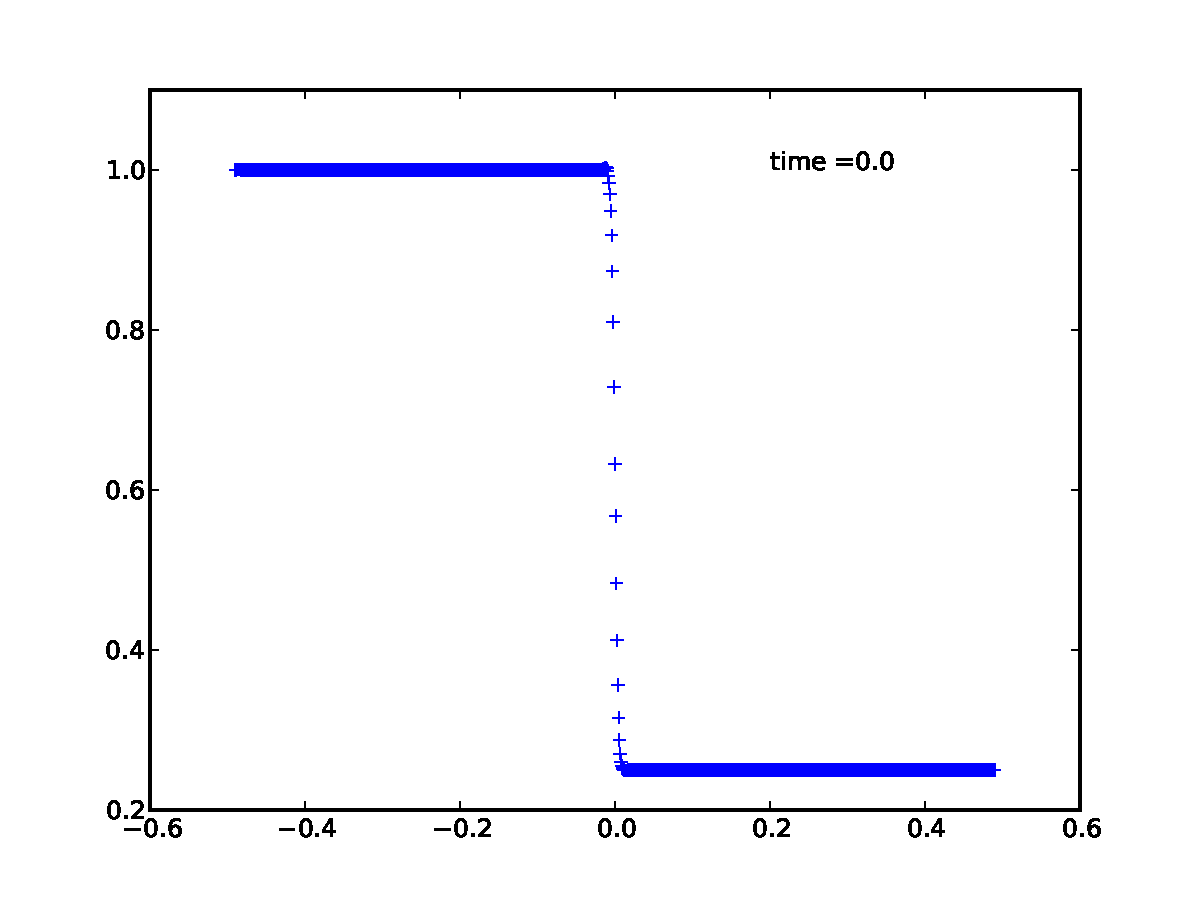
\includegraphics[width=0.45\textwidth]{Shock1}
	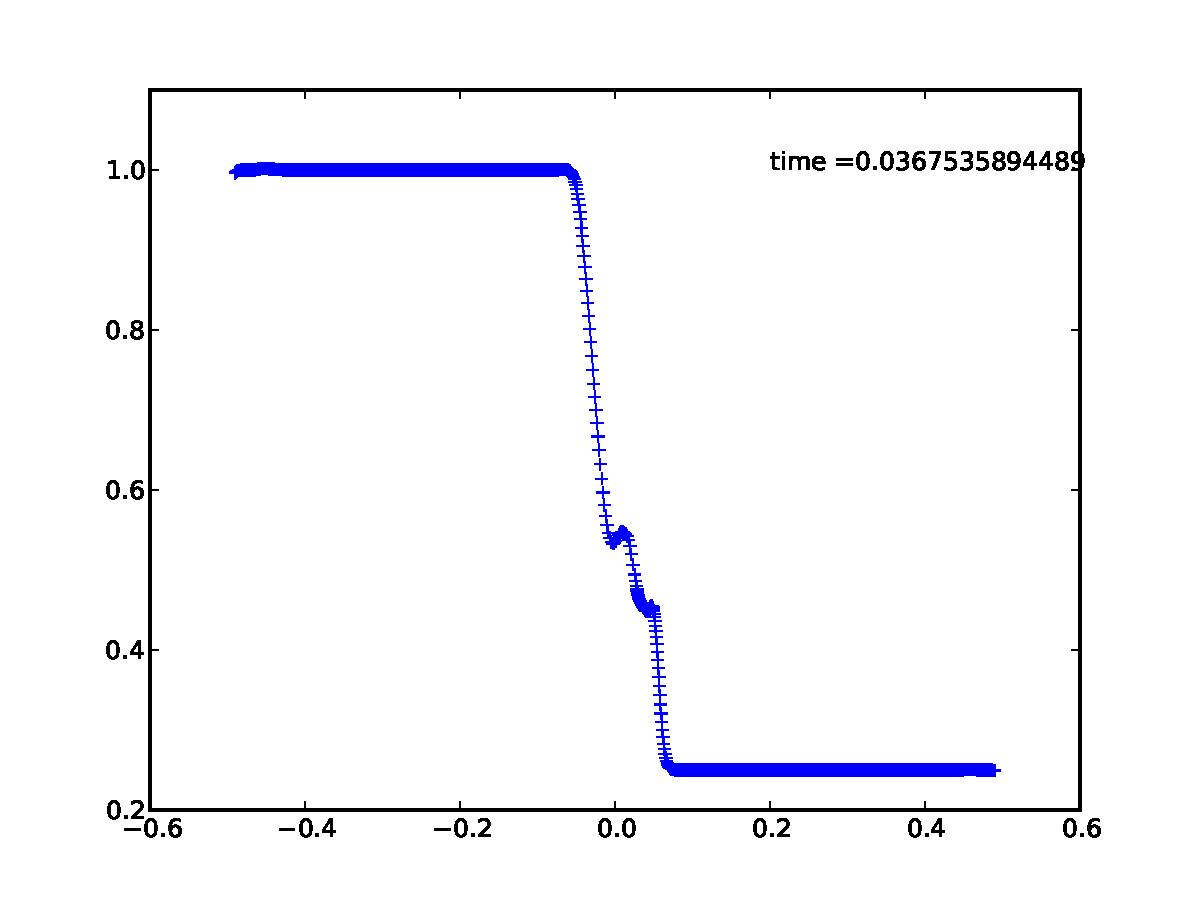
\includegraphics[width=0.45\textwidth]{Shock2} \\
	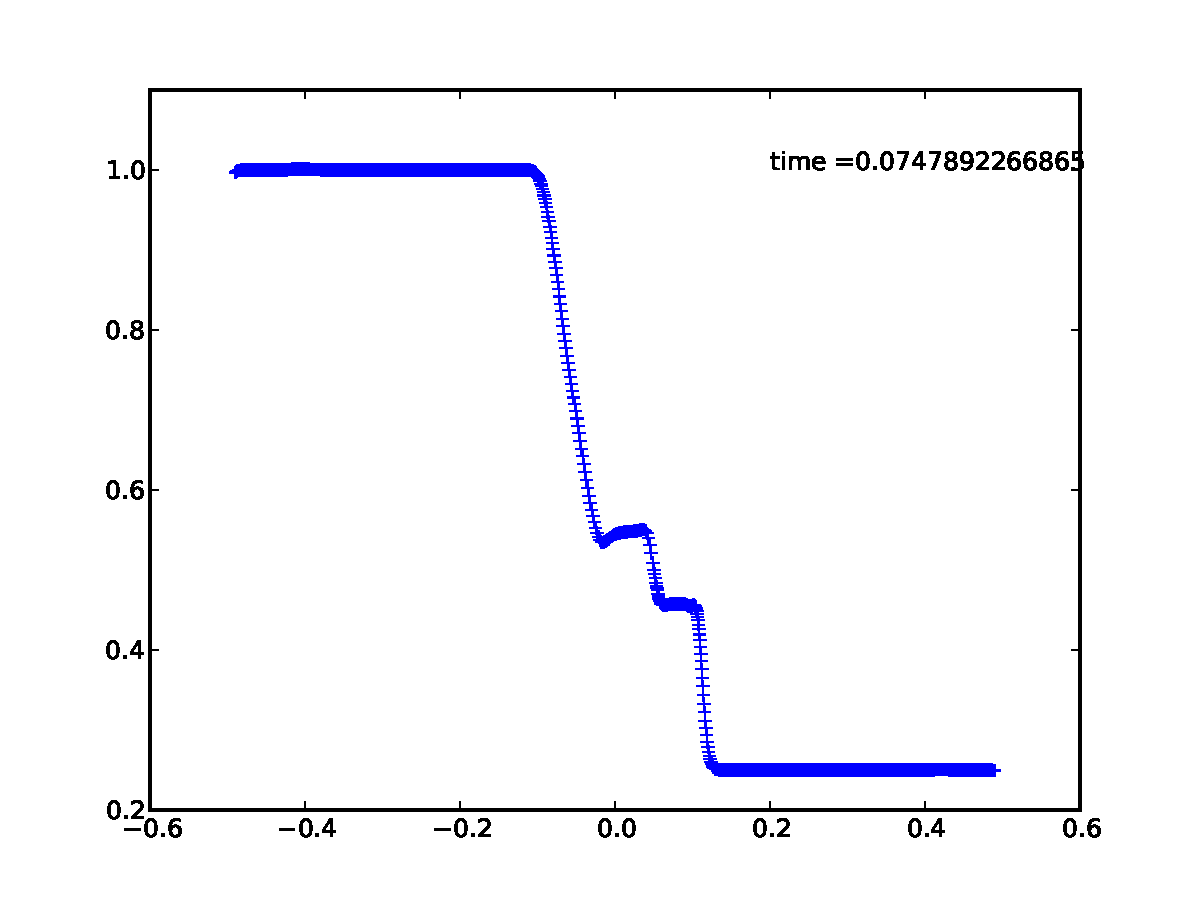
\includegraphics[width=0.45\textwidth]{Shock3}
	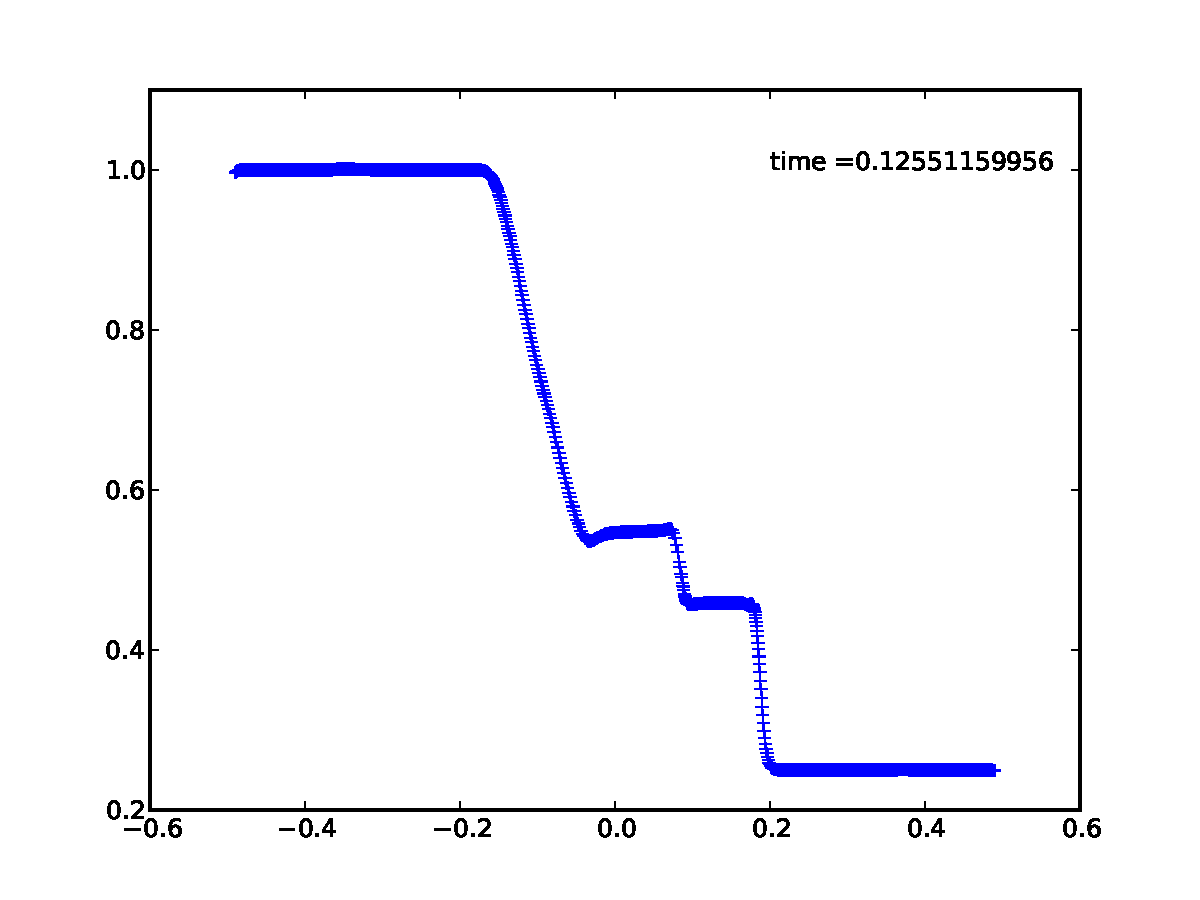
\includegraphics[width=0.45\textwidth]{Shock4} \\
	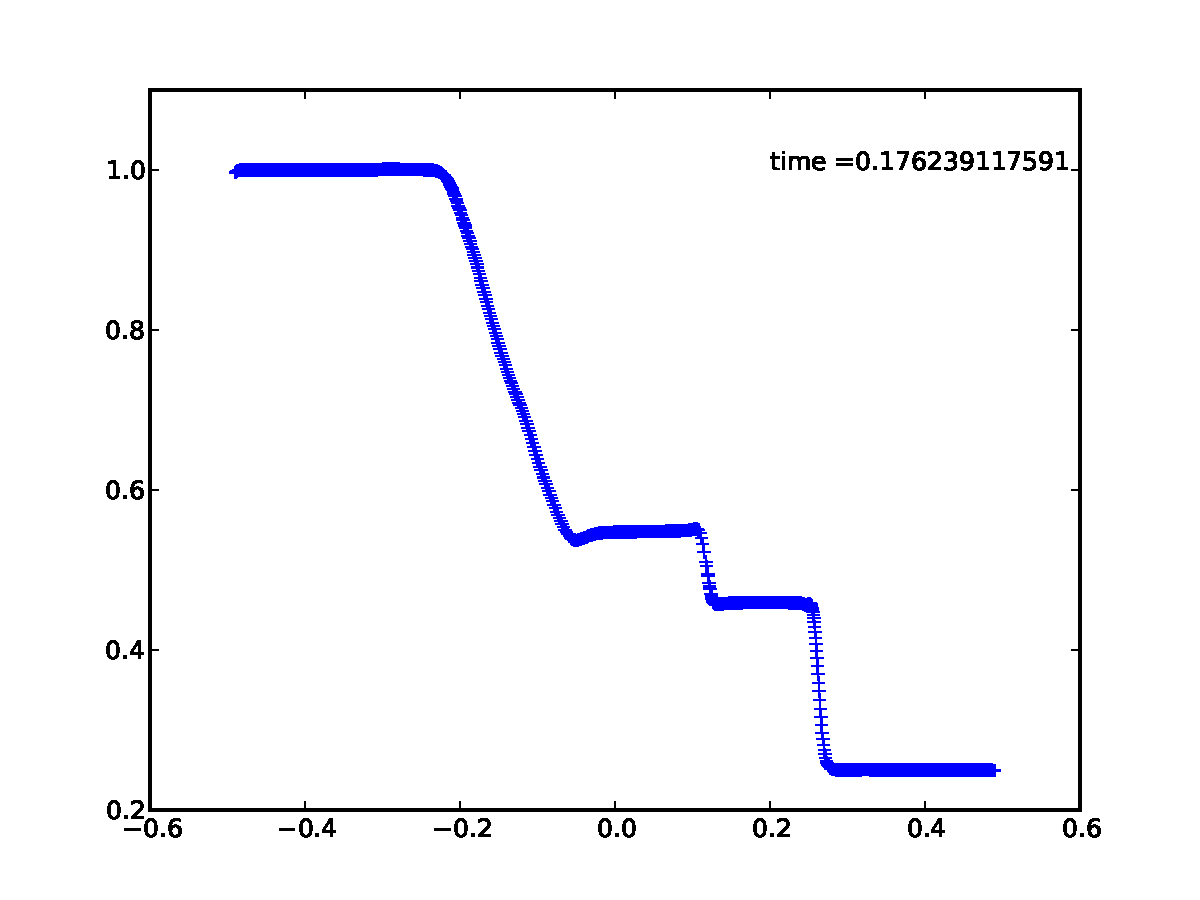
\includegraphics[width=0.45\textwidth]{Shock5}
	\includegraphics[width=0.45\textwidth]{Shockfinal}
\end{figure}	
\end{document}

